\section{Theoretical Background}
% \addcontentsline{toc}{section}{Theoretical Background}
\fancyhead[R]{Theoretical Background}

\subsection{Principles of Enzymology}
\label{sec:Principles of Enzymology}

Enzymology is the scientific study of enzymes, which are biological catalysts that accelerate biochemical reactions in living organisms. These macromolecules are essential for various cellular processes, including metabolism, DNA replication, and signal transduction. The understanding of enzyme structure, function, and kinetics is crucial for developing applications in biotechnology, medicine, and environmental science. \autocite{robinsonEnzymesPrinciplesBiotechnological2015}

Enzymes are classified based on the types of reactions they catalyze, according to a system established by the Enzyme Commission (EC). This classification system groups enzymes into six main classes, each with specific types of reactions they facilitate:

\begin{compactenum}
    \item \textbf{Oxidoreductases:} These enzymes catalyze oxidation-reduction reactions, where the transfer of electrons occurs between molecules. Examples include dehydrogenases and oxidases.
    \item \textbf{Transferases:} These enzymes transfer functional groups from one molecule to another. Examples include kinases, which transfer phosphate groups.
    \item \textbf{Hydrolases:} These enzymes catalyze the hydrolysis of various bonds, including ester, glycosidic, peptide, and others. Examples include proteases and lipases.
    \item \textbf{Lyases:} These enzymes add or remove groups to form double bonds, without hydrolysis or oxidation. Examples include decarboxylases and dehydratases.
    \item \textbf{Isomerases:} These enzymes catalyze the rearrangement of atoms within a molecule, leading to isomerization. Examples include racemases and epimerases.
    \item \textbf{Ligases:} These enzymes catalyze the joining of two molecules with the simultaneous hydrolysis of a diphosphate bond in ATP or a similar triphosphate. Examples include synthetases and carboxylases.
    
\end{compactenum}

For example, the enzyme tripeptide aminopeptidase has the EC number "3.4.11.4", where the first digit (3) represents the class (Hydrolases in this case), the second digit (4) represents the subclass (hydrolases that act on peptide bonds), the third digit (11) represents the sub-subclass (Hydrolases that cleave off the amino-terminal amino acid from a polypeptide), and the fourth digit (4) represents the serial number of the enzyme within the sub-subclass (Hydrolases that cleave off the amino-terminal end from a tripeptide). This systematic classification allows researchers to identify enzymes based on their catalytic activities and biochemical properties. \autocite{EnzymeNomenclatureRecommendations1994}
The distribution of EC numbers across the six classes is not uniform, with hydrolases being the most abundant class, reflecting the importance of hydrolysis in biological processes. The following figure shows the distribuion of EC numbers across all four levels of the classification system:

\begin{table}[hbt]
    \centering
    \begin{tabular}{@{}ll@{}}
    \toprule
    \textbf{EC Level} & \textbf{Number of classes} \\ \midrule
    1                 & 7                          \\
    2                 & 79                         \\
    3                 & 320                        \\
    4                 & 7876                       \\ \bottomrule
    \end{tabular}
    \caption{Distribution of EC numbers across different levels of the classification system.}
    \label{tab:ec-level-distribution}
\end{table}

Enzymes are not only classified based on their catalytic activities but also based on their biological functions. The three-dimensional (3D) structure of enzymes is fundamental to their function. Enzymes are composed of one or more polypeptide chains that fold into specific shapes to form the active site. The active site is where substrate molecules bind and undergo a chemical reaction. The enzyme structure serves as a scaffold to support and correctly position the active site for optimal catalytic activity. 

\begin{figure}[hbt]
    \centering
    \begin{minipage}[t]{.9\textwidth}
    \caption{Organisation of enzyme structure and lysozyme example.}
    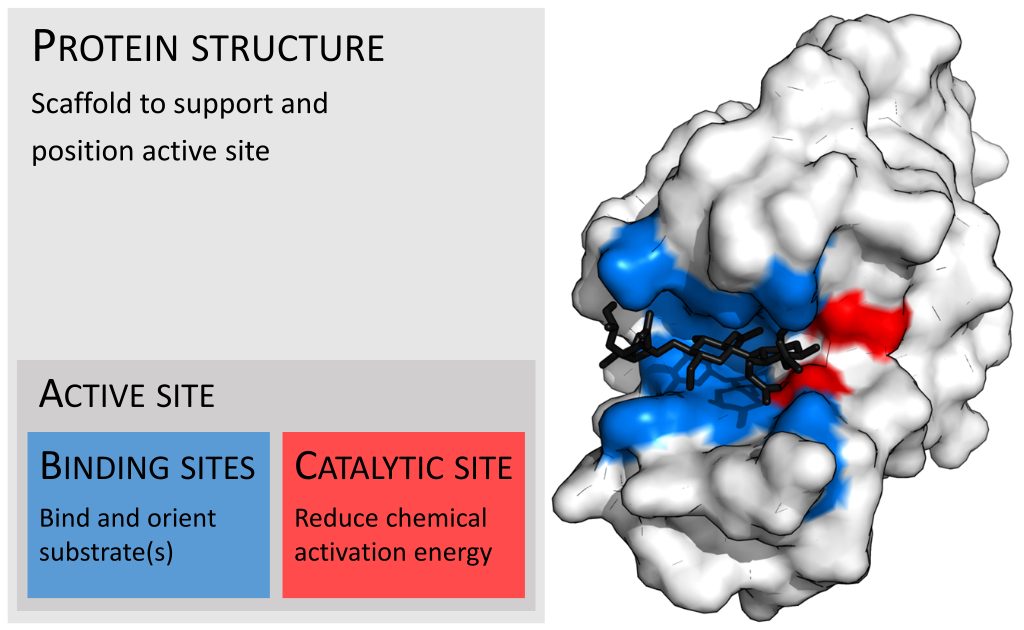
\includegraphics[width=1\textwidth]{img/EnzymeStructure.svg.png}\\
    \source{Thomas Shafee, CC BY 4.0 via Wikimedia Commons}
    \label{fig:EnzymeStructure}
    \end{minipage}
\end{figure}

\begin{itemize}
    \item \textbf{Protein Structure:} The overall structure of the enzyme provides the framework that supports and positions the active site. This structure is critical for the enzyme's stability and functionality. The enzyme's polypeptide chains fold into a unique 3D shape, creating a specific environment for the active site.
    \item \textbf{Active Site:} The active site includes two critical regions: binding sites and the catalytic site. The binding sites (highlighted in blue) are regions where substrates bind to the enzyme. These sites ensure that the substrates are properly oriented for the reaction. The catalytic site (highlighted in red) is the region where the chemical reaction occurs. The catalytic site often contains amino acids with specific functional groups that participate directly in the reaction, reducing the activation energy required for the reaction to proceed.
\end{itemize}

The Key-Lock Principle, first proposed by Emil Fischer in 1894, is a model for understanding the specificity of enzyme-substrate interactions. According to this principle, the enzyme (lock) has a specific active site shape that only fits a particular substrate (key). This model emphasizes the specificity of enzyme-substrate interactions and how enzymes are highly selective for their substrates. This principle is fundamental to understanding enzyme function and the mechanisms of catalysis. The specificity of these interactions is crucial for predicting enzyme activities because it determines the substrates that can bind to the enzyme and undergo catalysis.

\begin{figure}[hbt]
    \centering
    \begin{minipage}[t]{.8\textwidth}
    \caption{Lock-and-key model that explains the selectivity of enzymes}
    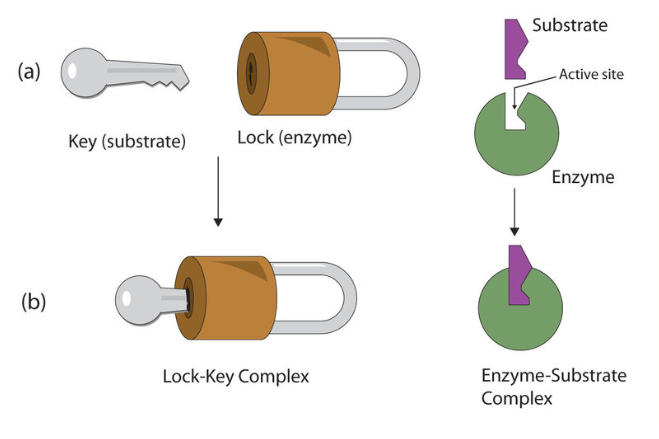
\includegraphics[width=1\textwidth]{img/key_lock_principle.png}\\
    \source{\autocite{poshyvailo-strubeModellingSimulationsEnzymecatalyzed2015a}}
    \label{fig:LockKeyPrinciple}
    \end{minipage}
\end{figure}

The precise arrangement of amino acids in the active site allows enzymes to be highly specific for their substrates, facilitating efficient catalysis. This specificity is a key feature that enables enzymes to perform their roles in various biochemical pathways with high precision. Understanding the structure-function relationship of enzymes is essential for predicting their activities.

\subsection{Fundamentals of Ligand Binding Site Prediction}
\label{sec:Fundamentals of Ligand Binding Site Prediction}

As mentioned earlier, enzymes interact with substrates at specific binding sites, where the catalytic reactions occur. Predicting these ligand-binding sites is crucial for understanding the enzyme function. Several computational methods have been developed to predict ligand-binding sites from protein structures, including geometric, physicochemical, and machine learning-based approaches.

One approach is P2Rank, a machine learning-based tool designed for the rapid and accurate prediction of ligand binding sites from protein structures. It employs a combination of geometric and physicochemical descriptors to analyze protein structures and predict the locations of potential binding sites. P2Rank uses a random forest algorithm, an ensemble learning method that constructs multiple decision trees during training and outputs the mode of the classes (classification) or mean prediction (regression) of the individual trees.

The tool focuses on the interactive parts of enzymes, particularly the ligand-binding sites and the specific amino acids involved. This detailed analysis allows for accurate predictions of enzyme classes and their associated degradation pathways. P2Rank's ability to quickly and accurately predict binding sites makes it a valuable tool for drug discovery and environmental bioremediation applications.

P2Rank leverages local chemical neighborhood features near the protein surface to infer potential binding sites for ligands. Here is an overview of the key steps involved in the P2Rank prediction process:

\begin{enumerate} 
    \item \textbf{Generation of Connolly Points}: Connolly Points are regularly spaced points generated on the protein’s Connolly surface, representing the solvent-accessible surface area of the protein. These points are generated using a numerical algorithm that ensures even spacing, typically with a solvent radius of 1.6 Å.
    \item \textbf{Calculation of Feature Descriptors}: Atomic Feature Vectors (AFVs) are calculated for each solvent-exposed heavy atom in the protein, describing various physico-chemical properties such as hydrophobicity, aromaticity, and more. These properties are projected onto the Connolly points using a distance-weighted approach, creating Connolly Feature Vectors (CFVs) for each point. The image shows Connolly Points (green dots) on the protein’s surface, where each point is associated with a Connolly Feature Vector (CFV).
    \begin{enumerate}
        \item Atomic Features: Features are inherited from the amino acid, including properties like hydrophobicity and polarity index. Additional features for AA atoms include H-Donor, H-Acceptor, and aromaticity.
        \item Aggregation of Feature Vectors: The CFV for each Connolly point is calculated by aggregating the AFVs of neighboring atoms using a distance-based weight function $w(d) = 1 - d / 6$.
    \end{enumerate}
        \begin{figure}[hbt]
            \centering
            \begin{minipage}[t]{.9\textwidth}
            \caption{Calculation of feature vectors for neighboring atoms in P2Rank.}
            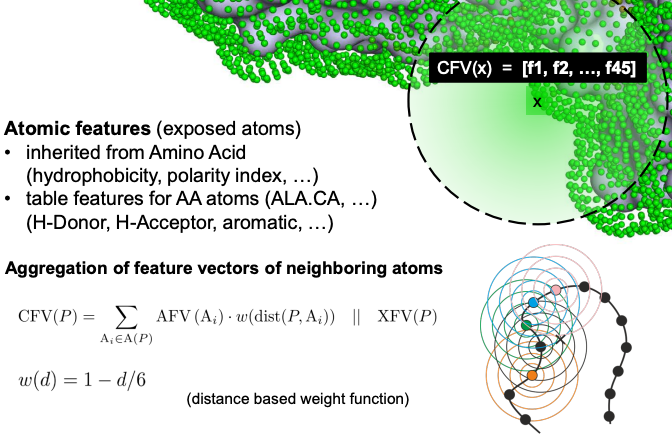
\includegraphics[width=1\textwidth]{img/slide_p2rank.png}\\
            \source{Radoslav Krivák and David Hoksza}
            \label{fig:p2rank}
            \end{minipage}
        \end{figure}
    \item \textbf{Ligandability Prediction}: A Random Forest classifier is used to predict the ligandability score for each Connolly point, indicating the likelihood that a point is part of a ligand-binding site.
    \item \textbf{Clustering}: Connolly points with high ligandability scores are clustered using a single-linkage clustering method, representing potential binding pockets on the protein surface.
    \item \textbf{Ranking}: Each predicted pocket is assigned a score based on the cumulative ligandability scores of its constituent points, helping prioritize the most likely binding sites for further analysis or docking studies.
\end{enumerate}

P2Rank's approach can significantly enhance the accuracy of predicting enzyme-mediated degradation of pesticides by providing detailed insights into the binding interactions at the molecular level. This integration of deep learning and enzyme analysis forms a robust framework for developing bioremediation strategies and understanding the environmental fate of various pollutants. \autocite{krivakP2RankMachineLearning2018}

\subsection{Introduction to Recurrent Neural Networks}
\label{sec:Introduction to Recurrent Neural Networks}

RNNs (RNNs) are a class of artificial neural networks designed to recognize patterns in sequences of data such as text, genomes, handwriting, and spoken words. Unlike traditional feedforward neural networks, RNNs have connections that form directed cycles, allowing information to persist. This makes them particularly powerful for tasks that involve sequential data, where the order of the data points matters. \autocite{RecurrentNeuralNetwork2024}

RNNs are designed to process sequences of data by maintaining a memory of previous inputs. This memory allows RNNs to make use of information from earlier in the sequence to influence the current processing step, which is essential for understanding context in sequential data. The fundamental difference between RNNs and traditional neural networks is the presence of loops in the network that enable the persistence of information across time steps.

RNNs are designed to process sequences of data by maintaining a memory of previous inputs. This memory allows RNNs to make use of information from earlier in the sequence to influence the current processing step, which is essential for understanding context in sequential data. The fundamental difference between RNNs and traditional neural networks is the presence of loops in the network that enable the persistence of information across time steps.

The basic structure of an RNN includes an input layer, a hidden layer with recurrent connections, and an output layer. At each time step, the hidden layer receives the input data and its own previous state, allowing it to retain and process information from previous steps in the sequence.

One of the key advancements in RNNs is the development of Long Short-Term Memory (LSTM) networks and Gated Recurrent Units (GRUs), which are designed to overcome the limitations of traditional RNNs, such as the vanishing gradient problem. These architectures use gating mechanisms to control the flow of information, making it easier to capture long-term dependencies in data.

In the context of bioinformatics, RNNs, particularly LSTMs and GRUs, are extensively used for sequence analysis tasks such as protein secondary structure prediction, gene expression analysis, and more. They are effective because they can handle the sequential nature of biological data and capture dependencies that span over long sequences. LSTM networks are a type of RNN that can learn long-term dependencies. They incorporate memory cells that can maintain their state over long periods. LSTMs have three main gates (input gate, forget gate, and output gate) that regulate the flow of information into and out of the memory cell, thus enabling the network to remember important information for longer durations. \autocite{hochreiterLongShortTermMemory1997}

The following image illustrates the basic structure of an RNN:

\begin{figure}[hbt]
    \centering
    \begin{minipage}[t]{\textwidth}
    \caption{A diagram for a one-unit RNN.}
    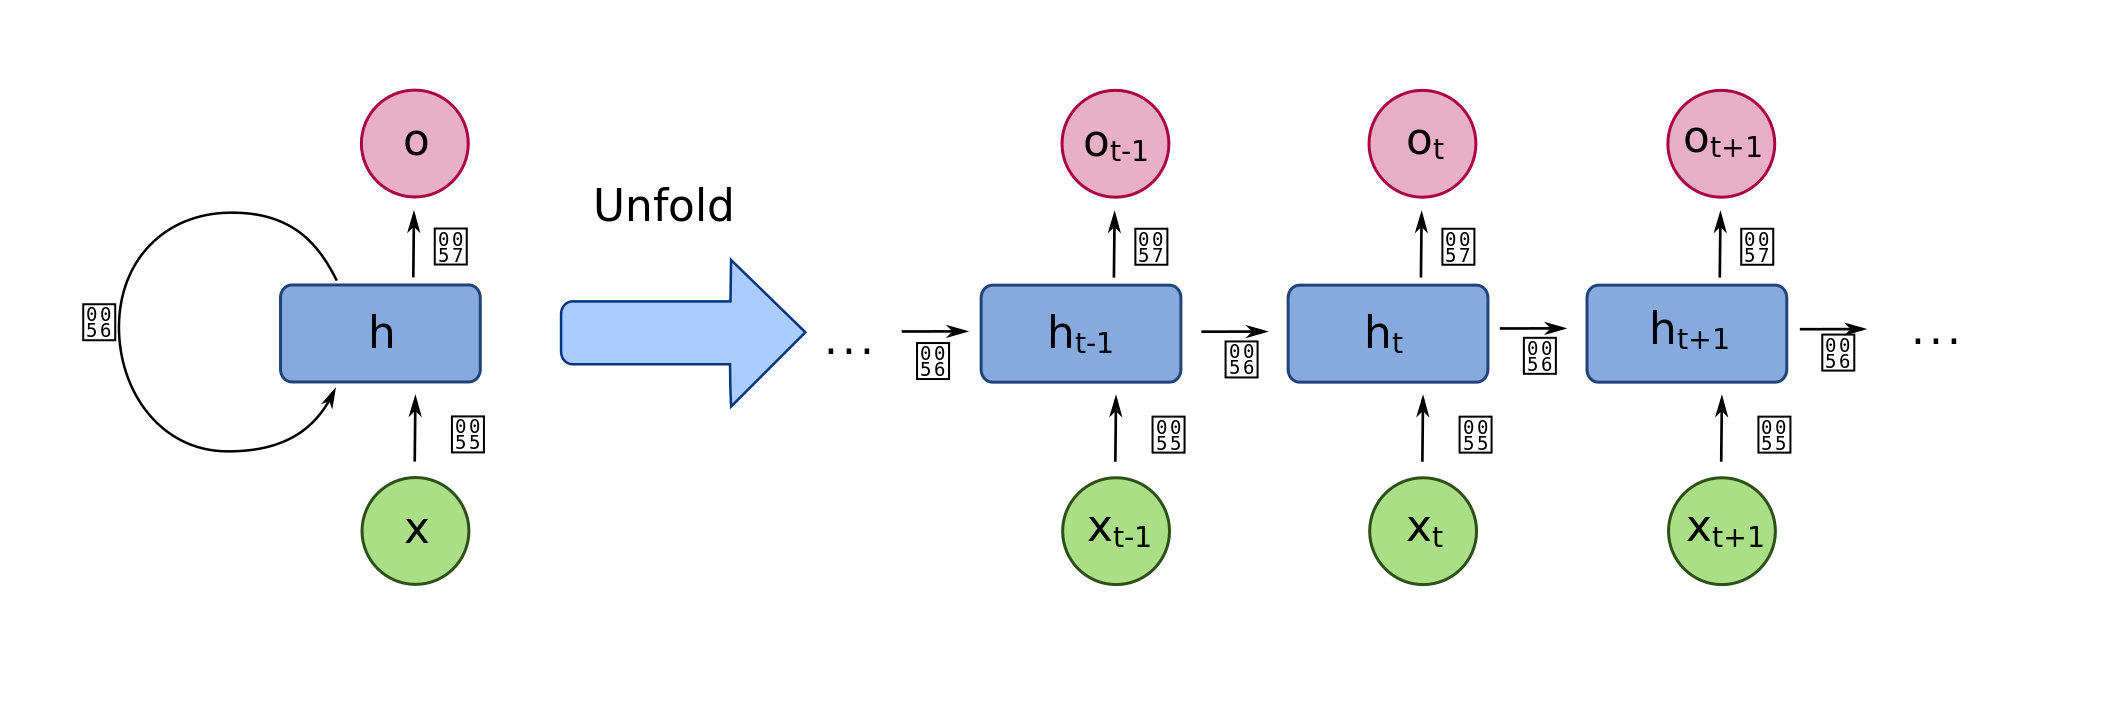
\includegraphics[width=1\textwidth]{img/Recurrent Neural Network Unfold.png}\\
    \source{fdeloche, CC BY-SA 4.0 via Wikimedia Commons}
    \label{fig:RNN}
    \end{minipage}
\end{figure}

\begin{enumerate}
    \item Input Sequence (x): The green circles represent the input data at different time steps ($ x_{t-1}, x_{t}, x_{t+1} $).
    \item Hidden State (h): The blue rectangles represent the hidden state of the network. At each time step, the hidden state (h) is updated based on the current input and the previous hidden state ($h_{t-1}, h_{t}, h_{t+1}$).
    \item Output Sequence (o): The pink circles represent the output of the network at each time step ($o_{t-1}, o_{t}, o_{t+1}$).
\end{enumerate}

The recurrent connection (arrow looping back) in the hidden state allows information to persist across time steps, enabling the network to maintain context and capture dependencies in the sequence data.

In this study, RNNs are employed for predicting the enzyme class based on the amino acid sequences of a ligand binding site. The sequential nature of the amino acid sequences makes RNNs well-suited for this task, as they can capture the dependencies and patterns in the data that are crucial for predicting enzyme classes accurately. Especially for complex and long sequences, RNNs, particularly LSTMs, are effective in learning the underlying structure and relationships in the data.

\subsection{Evaluation of Deep Learning Models}
\label{sec:Evaluation of Deep Learning Models}

When developing a deep learning model, it is crucial to compare its performance with other models and make necessary adjustments. This process ensures that the selected model is not only the best fit for the current dataset but also generalizes well to new data. By evaluating multiple models, it is possible to identify which model architecture and hyperparameters yield the best performance. This can be done through adjusting hyperparameters such as learning rate, batch size, and network depth to optimize model performance. Techniques like dropout, L2 regularization, and batch normalization can also be used to prevent overfitting and improve model generalizability. To access the generalizability of the model, it is essential to evaluate its performance on unseen data, typically through a validation set or cross-validation. Cross-Validation is a widely used technique for evaluating model performance by splitting the dataset into multiple subsets, training the model on different subsets, and testing it on the remaining data. This process helps assess the model's performance across different data partitions and provides a more robust estimate of its generalization capabilities.

The best-known cross-validation method is k-fold. he data is divided into $k$ equally sized folds. The model is trained $k$ times, each time using a diffrent fold as the validation set and the remaining $k-1$ folds as the training set. Cross-validation helps in understanding the variability of model performance and reduces the risk of overfitting. Repeating cross-validation multiple times, known as repeated cross-validation, can further enhance reliability. \autocite{krstajicCrossvalidationPitfallsWhen2014}

\begin{figure}[hbt]
    \centering
    \begin{minipage}[t]{.8\textwidth}
    \caption{Cross-validation workflow for evaluating deep learning models.}
    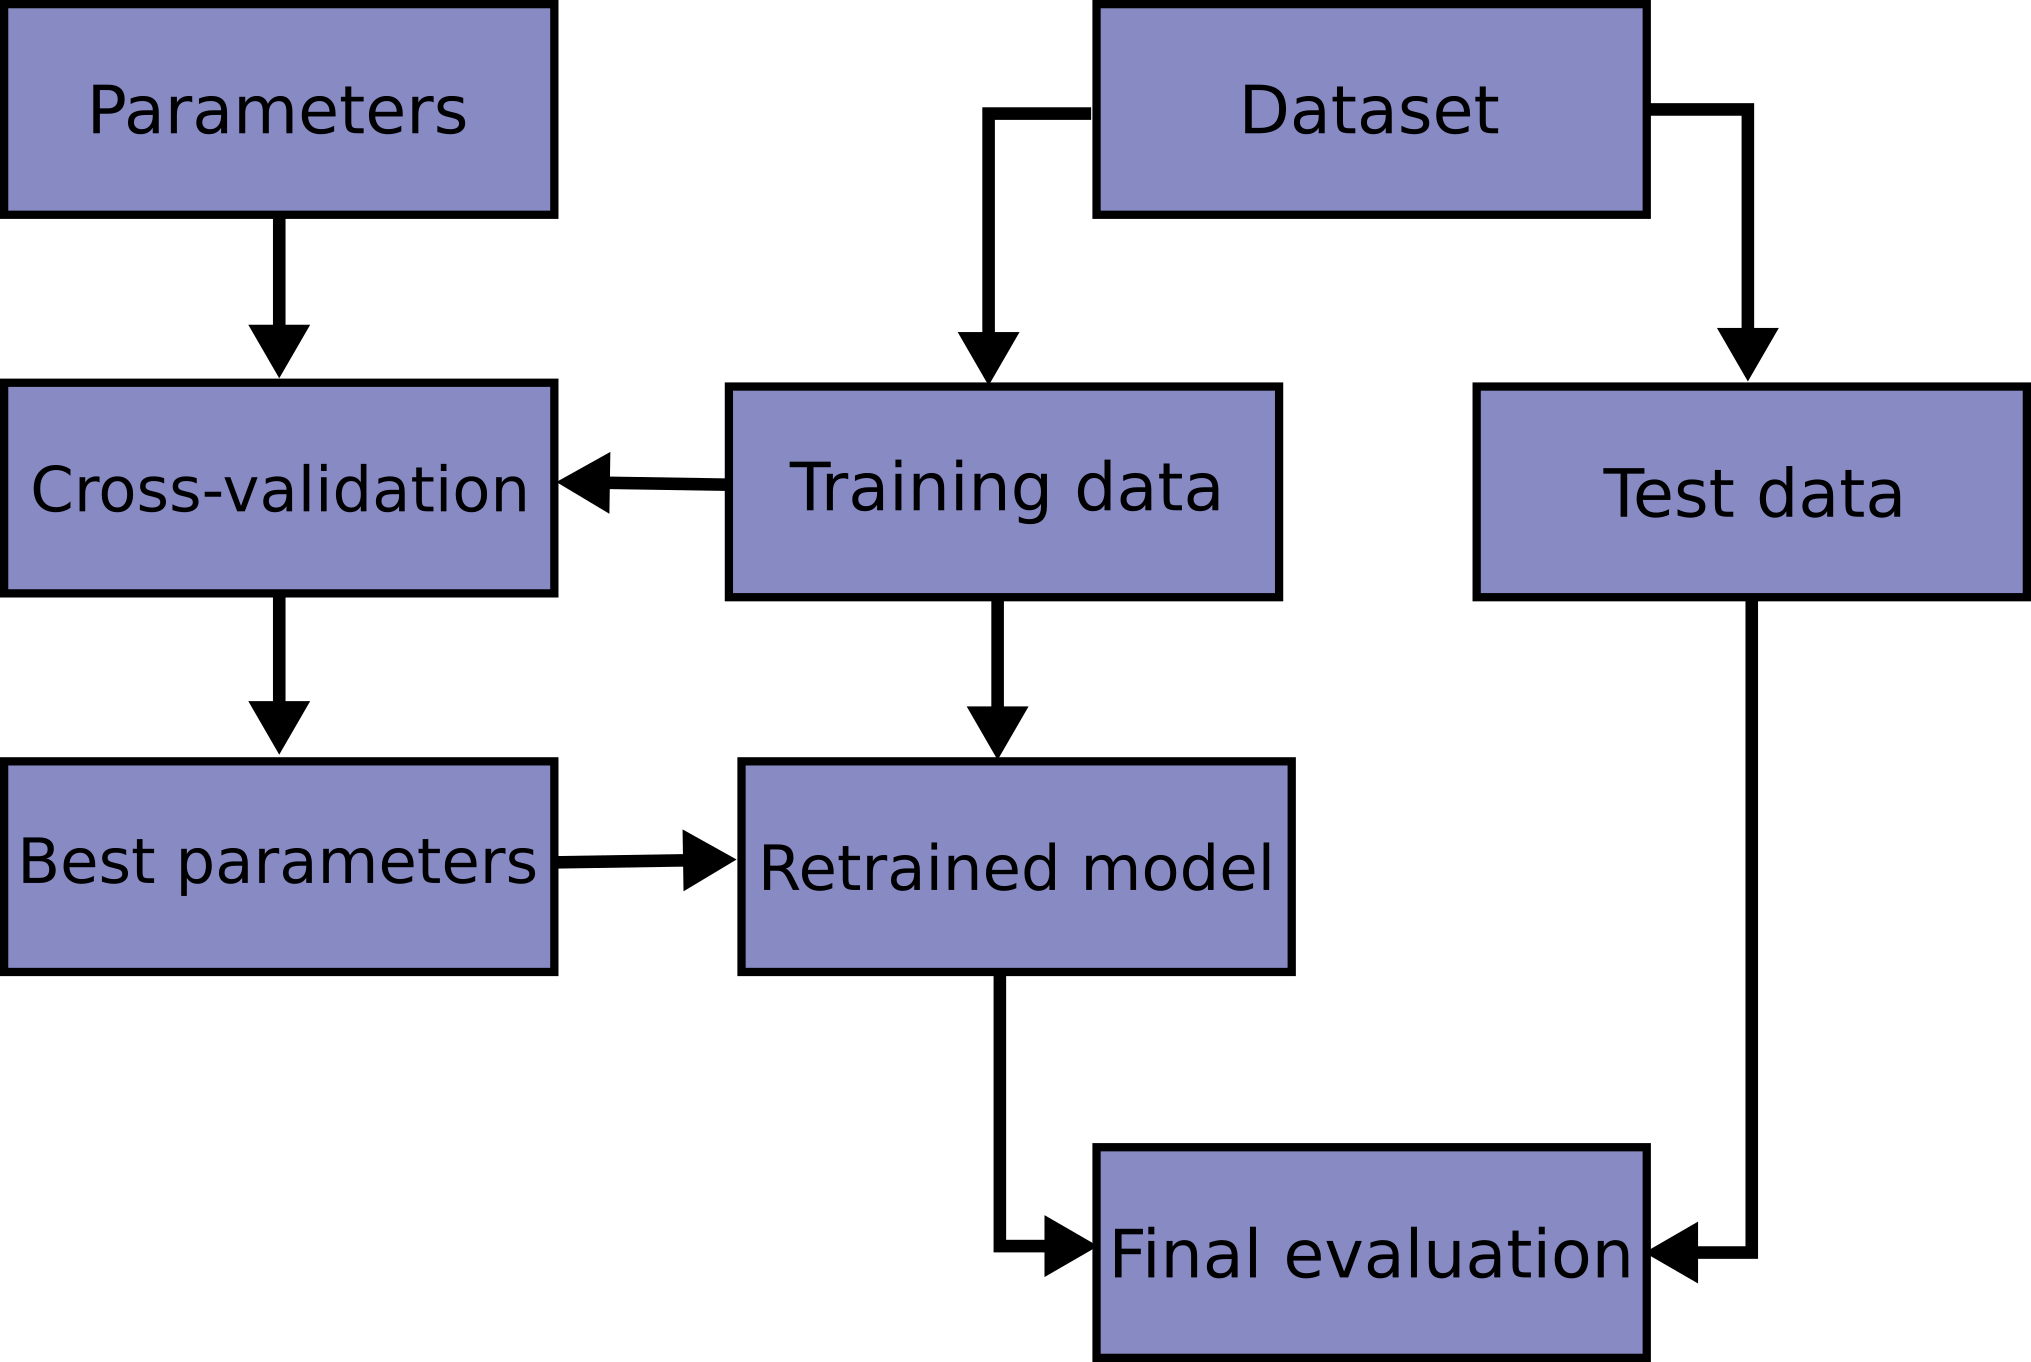
\includegraphics[width=.8\textwidth]{img/cross_validation_workflow.png}\\
    \source{scikit-learn Documentation}
    \label{fig:cross-validation-workflow}
    \end{minipage}
\end{figure}

Grid Search is a systematic way of tuning hyperparameters to find the optimal set that maximizes model performance. It involves defining a grid of possible hyperparameter values and exhaustively training and evaluating the model for each combination. For each combination of hyperparameters, the model is trained using the training data. The performance is than evaluated with a cross-validation for each hyperparameter combination. The hyperparameters that yield the best performance are selected as the optimal set. Grid Search is a powerful tool for fine-tuning deep learning models and optimizing their performance. \autocite{bergstraRandomSearchHyperParameter}

To effectively evaluate and compare models, various metrics are used: \autocite{PrecisionRecall2024} \autocite{Fscore2024} \autocite{AccuracyPrecision2024} 

\textbf{Accuracy:} Accuracy measures the proportion of correctly predicted instances out of the total instances. It is a straightforward metric but may not be reliable for imbalanced datasets.
\begin{equation}
    Accuracy = \frac{\text{Total Number of Predictions}}{\text{Number of Correct Predictions}}
\end{equation}

\textbf{Precision:} Precision indicates the accuracy of positive predictions, reflecting how many predicted positive instances are actually positive.
\begin{equation}
    Precision = \frac{\text{True Positives}}{\text{True Positives} + \text{False Positives}}
\end{equation}

\textbf{Recall:} Recall measures the model’s ability to identify all relevant instances, showing the proportion of actual positives correctly identified.
\begin{equation}
    Recall = \frac{\text{True Positives}}{\text{True Positives} + \text{False Negatives}}
\end{equation}

\textbf{F1 Score:} The F1 Score is the harmonic mean of precision and recall, providing a balanced measure when there is an uneven class distribution.
\begin{equation}
    F_1 = 2 \times \frac{\text{Precision} \times \text{Recall}}{\text{Precision} + \text{Recall}}
\end{equation}